



% Different Algortihms:
%
% - sequence-based:
%   - needle
% - folding and aligning
%   - LocARNA
% - Tree-based
%   - gardenia
%   - RNA StrAT
%   - RNAdistance
%   - RNAforester


\section{LocARNA}

\begin{frame}[c]{LocARNA - introduction}
    Two steps:
    \begin{itemize}
    \pause
    \item create base pair probability matrix using RNAfold
    \pause
    \item using these as guide for optimal alignment
    \pause
    \end{itemize}
    (folding and aligning)
\end{frame}


\section{Tree-based sequence alignment}

\subsection{gardenia}

\subsection{RNA StrAT}

\subsection{RNAdistance}

\subsection{RNAforester}



\section{Comparison}

\begin{frame}[c]{Run time Comparison}
    \center
    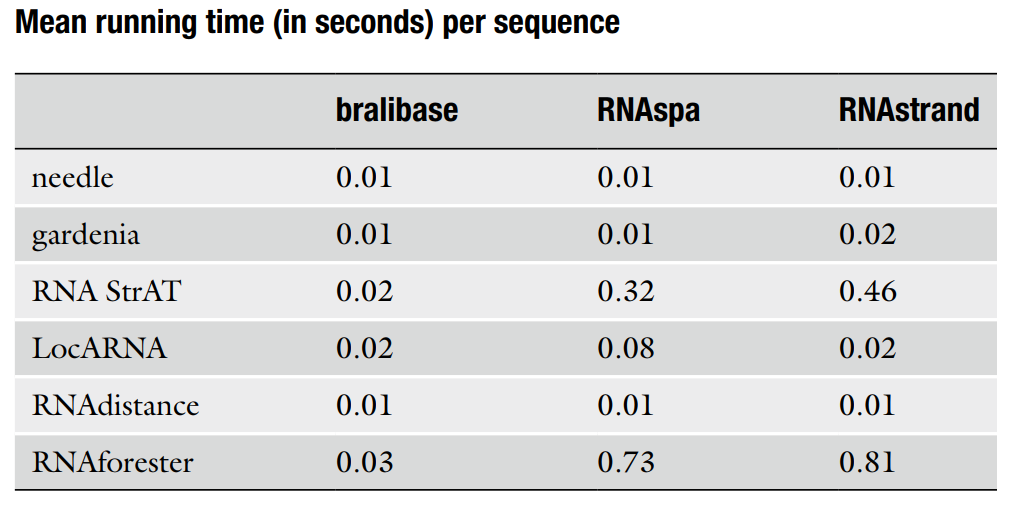
\includegraphics[width=\textwidth]{table}
\end{frame}

\begin{frame}[c]{}
    \center
    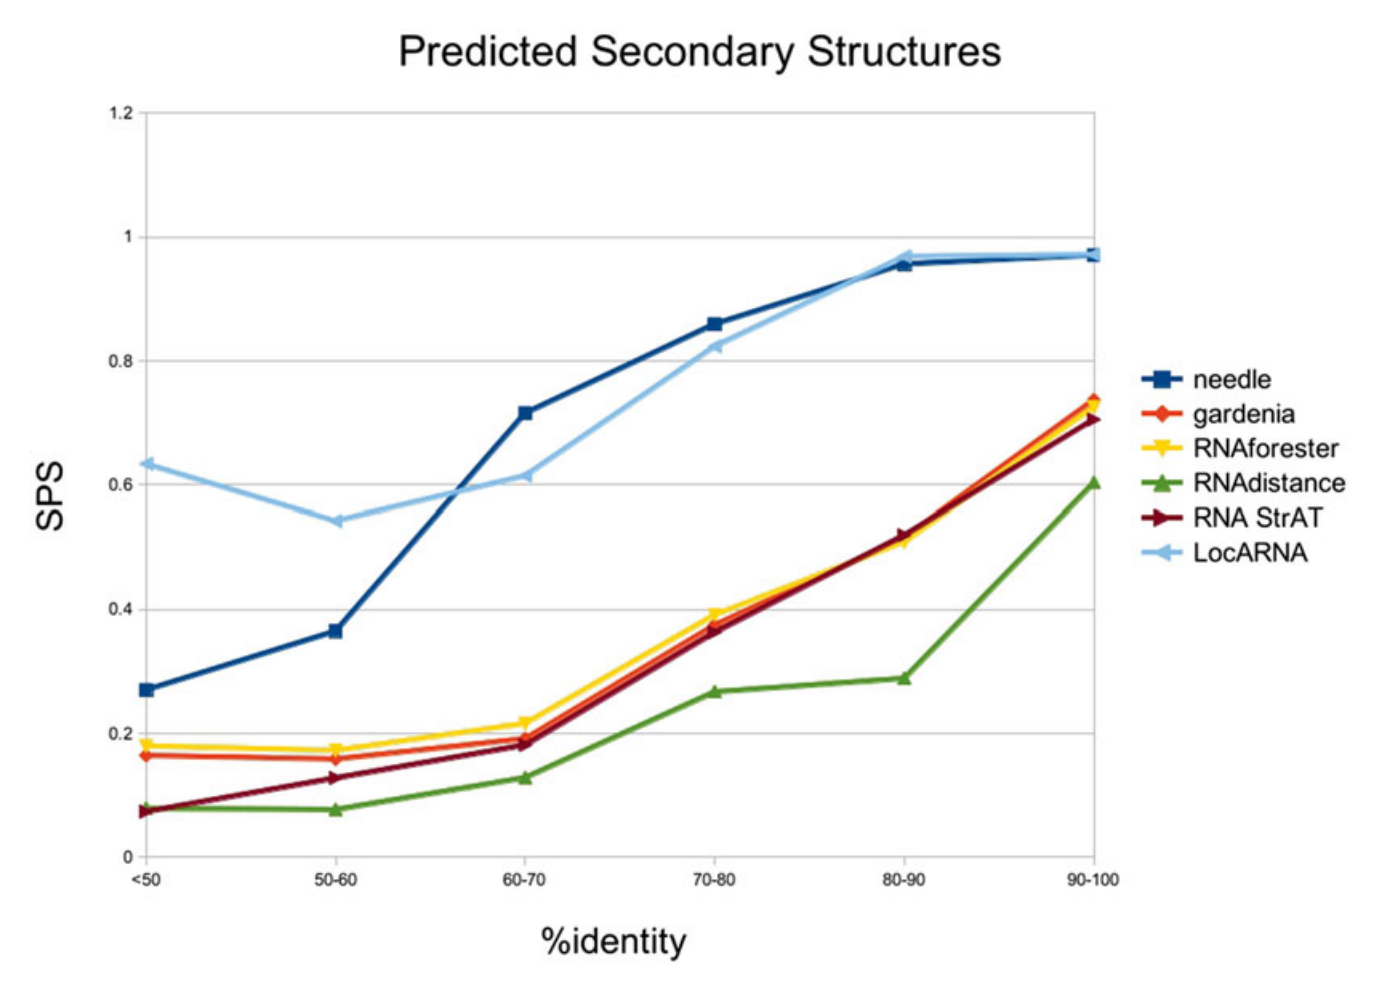
\includegraphics[width=\textwidth]{predicted}
\end{frame}

\begin{frame}[c]{}
    \center
    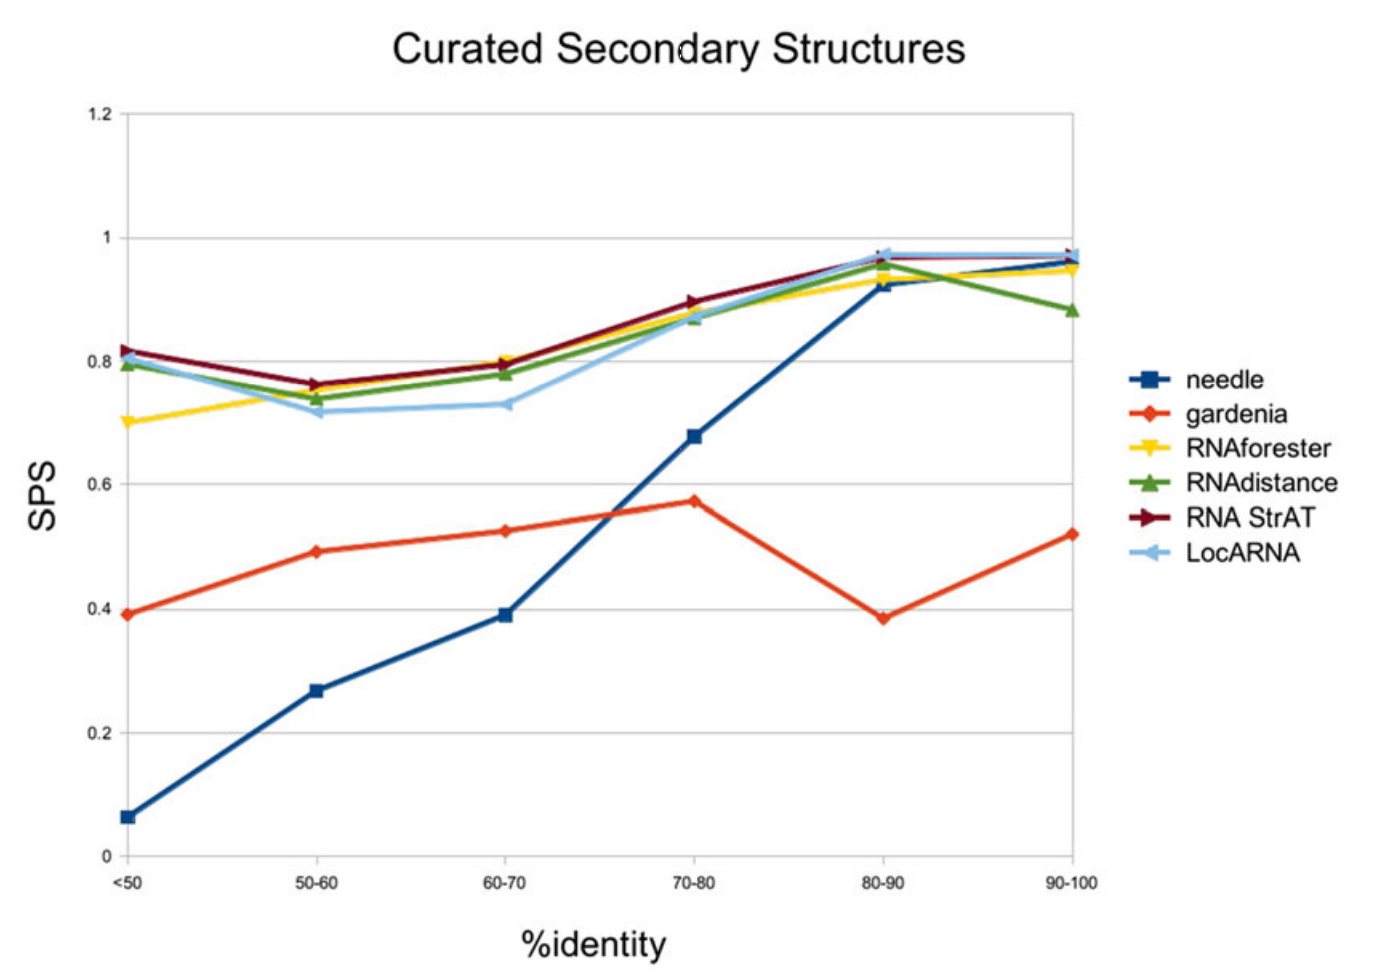
\includegraphics[width=\textwidth]{curated.png}
\end{frame}

\begin{frame}[c]{Proposed Workflow}
    \center
    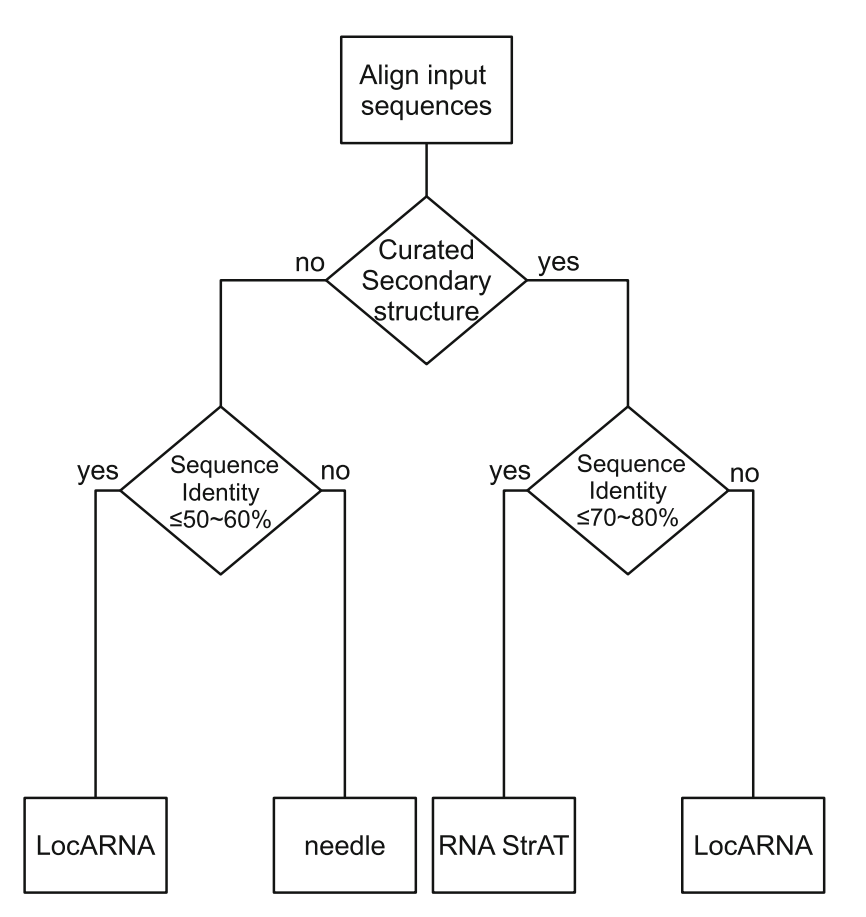
\includegraphics[height=.8\textheight]{flow}
\end{frame}



